\documentclass[a4paper,12pt]{article} 

% First, we usually want to set the margins of our document. For this we use the package geometry.
\usepackage[top = 2.5cm, bottom = 2.5cm, left = 2.5cm, right = 2.5cm]{geometry} 
\usepackage[T1]{fontenc}
\usepackage[utf8]{inputenc}

% The following two packages - multirow and booktabs - are needed to create nice looking tables.
\usepackage{multirow} % Multirow is for tables with multiple rows within one cell.
\usepackage{booktabs} % For even nicer tables.

% As we usually want to include some plots (.pdf files) we need a package for that.
\usepackage{graphicx} 

% The default setting of LaTeX is to indent new paragraphs. This is useful for articles. But not really nice for homework problem sets. The following command sets the indent to 0.
% \usepackage{setspace}
% \setlength{\parindent}{0in}
\usepackage{indentfirst}

% Package to place figures where you want them.
\usepackage{float}

% The fancyhdr package let's us create nice headers.
\usepackage{fancyhdr}

\usepackage{amsmath,amsthm,tikz}
\usetikzlibrary{automata,positioning}

% To make our document nice we want a header and number the pages in the footer.

\pagestyle{fancy} % With this command we can customize the header style.

\fancyhf{} % This makes sure we do not have other information in our header or footer.

\lhead{\footnotesize Discrete Mathematics(H): Homework 6}% \lhead puts text in the top left corner. \footnotesize sets our font to a smaller size.

%\rhead works just like \lhead (you can also use \chead)
\rhead{\footnotesize Mengxuan Wu} %<---- Fill in your lastnames.

% Similar commands work for the footer (\lfoot, \cfoot and \rfoot).
% We want to put our page number in the center.
\cfoot{\footnotesize \thepage} 

\begin{document}

\thispagestyle{empty} % This command disables the header on the first page. 

\begin{tabular}{p{15.5cm}}
{\large \bf Discrete Mathematics(H)} \\
Southern University of Science and Technology \\ Mengxuan Wu \\ 12212006 \\
\hline
\\
\end{tabular}

\vspace*{0.3cm} %add some vertical space in between the line and our title.

\begin{center}
	{\Large \bf Assignment 6}
	\vspace{2mm}

	{\bf Mengxuan Wu}
		
\end{center}  

\vspace{0.4cm}

\section*{Q.1}

\textbf{Symmetric:}

Since $G$ is a simple graph, every edge is undirected.
Hence, an edge associated to $\{u,v\}$ is also associated to $\{v,u\}$.
Then, if $uRv$, then there is an edge associated to $\{u,v\}$, and there is an edge associated to $\{v,u\}$, then $vRu$.
Therefore, $R$ is symmetric.

\textbf{Irreflexive:}

Since $G$ is a simple graph, there is no loop in $G$.
Hence, there is no edge associated to $\{u,u\}$.
Then, if $uRu$, then there is an edge associated to $\{u,u\}$, which is a contradiction.
Therefore, $R$ is irreflexive.

\section*{Q.2}

\begin{proof}
$ $

Let $a$ and $b$ be two arbitrary vertices in $G$. 

If there is an edge between $a$ and $b$, then there is a path between $a$ and $b$.

If there is no edge between $a$ and $b$, then we can find a vertex $c$ that is connected to both $a$ and $b$:

Let the subgraph $G_a$ be the graph contains vertices $a$ and $N(a)$.
Let the subgraph $G_b$ be the graph contains vertices $b$ and $N(b)$.

Since the degree of $a$ is at least $\frac{n-1}{2}$, the number of vertices in $G_a$ is at least $\frac{n-1}{2}+1=\frac{n+1}{2}$, and so is the number of vertices in $G_b$.
Hence, the sum of the number of vertices in $G_a$ and $G_b$ is at least $n+1$.
By the pigeonhole principle, there must be at least one vertex that is in both $G_a$ and $G_b$.

Let this vertex be $c$. 
Since there is no edge between $a$ and $b$, we know $a$ is not in $G_b$ and $b$ is not in $G_a$, thus $c$ is not $a$ or $b$.
And there is a path from $a$ to $c$ and a path from $b$ to $c$.
Therefore, there is a path from $a$ to $b$.

Since $a$ and $b$ are arbitrary, there is a path between any two vertices in $G$.
Therefore, $G$ is connected.
\end{proof}

\section*{Q.3}

\subsection*{(a)}

\begin{center}
	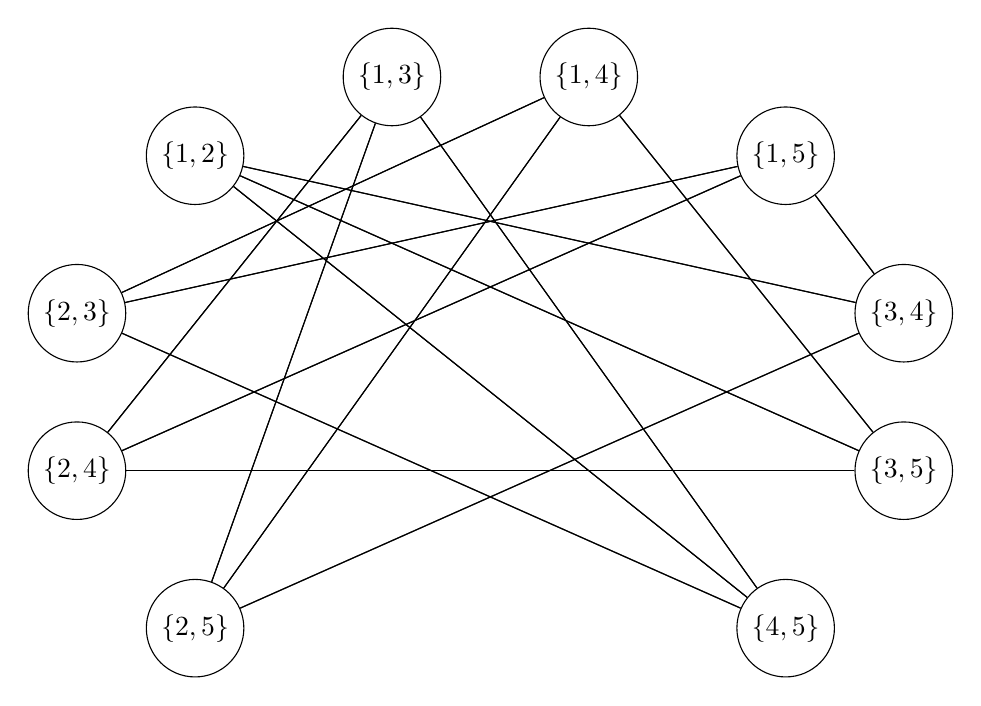
\begin{tikzpicture}[auto]
		\draw (-1,-1) node [state] (12){$\{1,2\}$};
		\draw (1.5,0) node [state] (13){$\{1,3\}$};
		\draw (4,0) node [state] (14){$\{1,4\}$};
		\draw (6.5,-1) node [state] (15){$\{1,5\}$};
		\draw (-2.5,-3) node [state] (23){$\{2,3\}$};
		\draw (-2.5,-5) node [state] (24){$\{2,4\}$};
		\draw (-1,-7) node [state] (25){$\{2,5\}$};
		\draw (8,-3) node [state] (34){$\{3,4\}$};
		\draw (8,-5) node [state] (35){$\{3,5\}$};
		\draw (6.5,-7) node [state] (45){$\{4,5\}$};

		\draw
		(12) edge (34)
			 edge (35)
			 edge (45)
		(13) edge (24)
			 edge (25)
			 edge (45)
		(14) edge (23)
			 edge (25)
			 edge (35)
		(15) edge (23)
		     edge (24)
			 edge (34)
		(23) edge (14)
			 edge (15)
			 edge (45)
		(24) edge (13)
			 edge (35)
			 edge (15)
		(25) edge (13)
			 edge (34)
			 edge (14)
		(34) edge (12)
			 edge (25)
			 edge (15)
		(35) edge (12)
			 edge (24)
			 edge (14)
		(45) edge (12)
			 edge (23)
			 edge (13);
		;
	\end{tikzpicture}
\end{center}

\subsection*{(b)}

The degree of each vertex in $G_n$ is $\binom{n-2}{2}$.

\begin{proof}
$ $

Each vertex is a set of two distinct integers from 1 to $n$.
Since each vertex can only connect to vertices that have no common elements with it, there are $n-2$ elements that can be chosen from.
Since each vertex is a set of two elements, there are $\binom{n-2}{2}$ vertices that can be connected to each vertex.
\end{proof}

\section*{Q.4}

\subsection*{(a)}

\begin{center}
	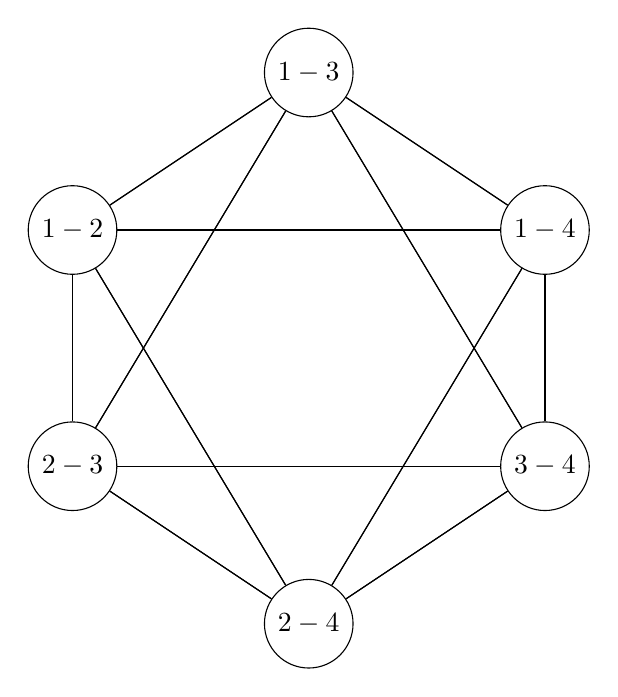
\begin{tikzpicture}[auto]
		\draw (0,0) node [state] (12){$1-2$};
		\draw (3,2) node [state] (13){$1-3$};
		\draw (6,0) node [state] (14){$1-4$};
		\draw (0,-3) node [state] (23){$2-3$};
		\draw (3,-5) node [state] (24){$2-4$};
		\draw (6,-3) node [state] (34){$3-4$};

		\draw
		(12) edge (13)
			 edge (14)
			 edge (23)
			 edge (24)
		(13) edge (14)
			 edge (12)
			 edge (23)
			 edge (34)
		(14) edge (12)
			 edge (13)
			 edge (24)
			 edge (34)
		(23) edge (12)
			 edge (13)
			 edge (24)
			 edge (34)
		(24) edge (12)
			 edge (14)
			 edge (23)
			 edge (34)
		(34) edge (13)
			 edge (14)
			 edge (23)
			 edge (24);
		;
	\end{tikzpicture}
\end{center}

\subsection*{(b)}

The number of edges in $G'$ is $\sum_{v\in V} \binom{deg(v)}{2}$.

\begin{proof}
$ $

Let $v$ be a vertex in $G$ with degree $k$.
Hence, there are $k$ edges connected to $v$.
For any two edges connected to $v$, we draw an edge in $G'$, this will produce $\binom{k}{2}$ edges.
In total this will produce $\sum_{v\in V} \binom{deg(v)}{2}$ edges in $G'$.
\end{proof}

\section*{Q.5}

\subsection*{(1)}

\begin{proof}
$ $

\textbf{Necessary condition:}

Let $v$ be a vertex in $N(A \cup B)$.

Hence, $v$ is connected to at least one vertex in $A \cup B$.
Without loss of generality, let $v$ be connected to $a \in A$.
Then $v \in N(A)$.
Hence, $v \in N(A) \cup N(B)$.

Therefore, $N(A \cup B) \subseteq N(A) \cup N(B)$.

\textbf{Sufficient condition:}

Let $v$ be a vertex in $N(A) \cup N(B)$.

Hence, $v$ is connected to at least one vertex in $A$ or $B$.
Without loss of generality, let $v$ be connected to $a \in A$.
Since $a \in A$, $a \in A \cup B$.
Then $v \in N(A \cup B)$.

Therefore, $N(A) \cup N(B) \subseteq N(A \cup B)$.

In all, $N(A \cup B) = N(A) \cup N(B)$.
\end{proof}

\subsection*{(2)}

Let $v$ be a vertex in $N(A \cap B)$.

Suppose $v$ is connected to vertex $a$ where $a \in A \cap B$, then $a \in A$ and $a \in B$.
Then $v \in N(A)$ and $v \in N(B)$.
Hence, $v \in N(A) \cap N(B)$.

However, the converse is not true.
Let the graph be:

\begin{center}
	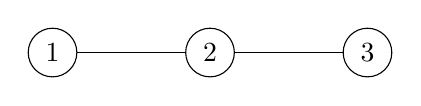
\begin{tikzpicture}
		\draw (0,0) node [circle, draw] (1) {1};
		\draw (2,0) node [circle, draw] (2) {2};
		\draw (4,0) node [circle, draw] (3) {3};

		\draw 
		(1) edge (2)
		(2) edge (3);
	\end{tikzpicture}
\end{center}

Let $A$ be vertex 1 and $B$ be vertex 3, then $A \cap B = \emptyset$.
Then $N(A \cap B) = \emptyset \neq \{2\} = N(A) \cap N(B)$.

\section*{Q.6}

\begin{proof}[Proof by contradiction]
$ $

By observation, we can see that each connected component of a bipartite graph is still bipartite.
And removing an edge will only affect the connected component that the edge is in, since an edge can only connect two vertices.
Hence, without loss of generality, we can assume that $G$ is connected.

Suppose that $e$ is a bridge in $G$.
Then we can split $G$ into two connected components $G_1$ and $G_2$ by removing $e$.
Let's focus on $G_1$.
Since $G_1$ is bipartite, we can color the vertices in $G_1$ with two colors, say red and blue.
And assume that there are $r$ red vertices and $b$ blue vertices in $G_1$.
Without loss of generality, let $e$ be connected to a red vertex.

Then, in $G_1$, the number of edges connected to red vertices is $k(r-1) + k-1$.
And the number of edges connected to blue vertices is $kb$.
Since $G_1$ is bipartite, $k(r-1) + k-1 = kb$.
Hence, $k(r-b) = 1$.

Since $k \geq 2$, it is impossible to have $k(r-b) = 1$.
There is a contradiction.

Therefore, $e$ is not a bridge in $G$.
And since $e$ is arbitrary, there is no bridge in $G$.
\end{proof}

\section*{Q.7}

\subsection*{(a)}

There is no cycle of length 1. 
Because a cycle of length 1 is a loop, and it means that there is a game between a player and himself, which is impossible.

There is no cycle of length 2.
Because a cycle of length 2 means that there are two games between two players, but there is only one game between any two players.

\subsection*{(b)}

\subsubsection*{(i)}

The ``beats'' relation is always antisymmetric.
Because there is only one game between any two players with no tie, then it is impossible to have $a$ beats $b$ and $b$ beats $a$.
Hence, there is no possibility that $aRb$ and $bRa$, which means that $R$ is antisymmetric.

\subsubsection*{(ii)}

The ``beats'' relation is never reflexive.
Because there is no game between a player and himself, then it is impossible to have $aRa$.
Then there is no possibility that $R$ is reflexive.

\subsubsection*{(iii)}

The ``beats'' relation is always irreflexive.
Because there is no game between a player and himself, then it is impossible to have $aRa$.
Then the only possibility is that $R$ is irreflexive.

\subsubsection*{(iv)}

The ``beats'' relation is sometimes transitive.
For example, if there are three players $a$, $b$ and $c$.
If $a$ beats $b$, $b$ beats $c$ and $a$ beats $c$, then $R$ is transitive.
However, if $a$ beats $b$, $b$ beats $c$ and $c$ beats $a$, then $R$ is not transitive.
Since the transitive property of $R$ will require that $a$ beats $c$ based on the fact that $a$ beats $b$ and $b$ beats $c$, but $c$ beats $a$.

\subsection*{(c)}

The tournament satisfies strict total order. (requires irreflexive instead of reflexive)

\textbf{Irreflexive and antisymmetric:}
The relation is always irreflexive as shown in (b)(iii), and it is always antisymmetric as shown in (b)(i).

\textbf{Transitive:}
\begin{proof}[Lemma]
$ $

\textit{If the tournament graph has a cycle, then there exists a cycle of length 3.}

It has proved that the graph has no cycle of length 1 or 2 in (a).
When $n = 3$, the lemma is trivial.
When $n > 3$, we can prove it by induction.

For a cycle of length $n > 3$, we can always find a cycle of length $n-1$ or 3.
Let $v_1 \rightarrow v_2 \rightarrow v_3 \rightarrow \cdots \rightarrow v_n \rightarrow v_1$ be a cycle in the tournament graph.
We can see that the graph is a complete graph because there is a game between any two players.
Then there is an edge between $v_1$ and $v_3$.
If the edge is $v_1 \rightarrow v_3$, then we can find a cycle $v_1 \rightarrow v_3 \rightarrow \cdots \rightarrow v_n \rightarrow v_1$, whose length is $n-1$.
If the edge is $v_3 \rightarrow v_1$, then we can find a cycle $v_1 \rightarrow v_2 \rightarrow v_3 \rightarrow v_1$, whose length is 3.
We repeat this process until we find a cycle of length 3.
\end{proof}

By the lemma above, we know that if the tournament graph has no cycle of length 3, then it has no cycle.
Then for any arbitrary three vertices $a$, $b$ and $c$, let $a$ beats $b$, $b$ beats $c$.
Since there is no cycle and the graph is a complete graph, $a$ must beats $c$.
Hence, the relation is transitive.

\textbf{Comparable:}

Since there is a game between any two players with no tie, then for any two vertices $a$ and $b$, either $a$ beats $b$ or $b$ beats $a$.
Hence, the relation is comparable.

\section*{Q.8}

\subsection*{(i)}

The minimal length of a path from $u$ to $v$ is the number of edges in the path.
If $u$ and $v$ is the same vertex, then the minimal length of a path from $u$ to $v$ is 0.
If they are not the same vertex, since the graph is connected, we can always find a path from $u$ to $v$.
Hence, $dist(u,v) \geq 0$.

\subsection*{(ii)}

The distance between $u$ and $v$ is the same as the distance between $v$ and $u$.
Because the minimal length path from $u$ to $v$ is the same as the minimal length path from $v$ to $u$.

\subsection*{(iii)}

If $dist(u,v) > dist(u,w) + dist(w,v)$, then the minimal length path from $u$ to $v$ is not the shortest path.
It can be improved by going from $u$ to $w$ and then from $w$ to $v$.
Hence, $dist(u,v) \leq dist(u,w) + dist(w,v)$.

\section*{Q.9}

These two graphs are not isomorphic.

In graph $G$, all vertices with degree 3 have two neighbors with degree 3 and one neighbor with degree 2.
However, in graph $H$, all vertices with degree 3 have one neighbors with degree 3 and two neighbor with degree 2.

\section*{Q.10}

\textbf{Reflexive:}

The isomorphism relation is reflexive.
For any graph, we can define a function $f$ that maps each vertex to itself.
Since $f$ is a bijection, $f$ is an isomorphism.

\textbf{Symmetric:}

The isomorphism relation is symmetric.
Since the function $f$ is a bijection, we can define a function $f^{-1}$ that maps each vertex to its inverse.
And $f^{-1}$ is a bijection, $f^{-1}$ is an isomorphism.

\textbf{Transitive:}

The isomorphism relation is transitive.
For three graphs $G_1$, $G_2$ and $G_3$, if $G_1$ is isomorphic to $G_2$ and $G_2$ is isomorphic to $G_3$, then there are two bijections $f$ and $g$ that maps $G_1$ to $G_2$ and $G_2$ to $G_3$.
Then we can define a function $h = g \circ f$ that maps $G_1$ to $G_3$.
Since $h$ is a bijection, $h$ is an isomorphism.

\section*{Q.11}

\begin{proof}[Disproof]
$ $

Let $G_1$, $H_1$, $G_2$ and $H_2$ be as shown in the figure below:
\begin{center}
	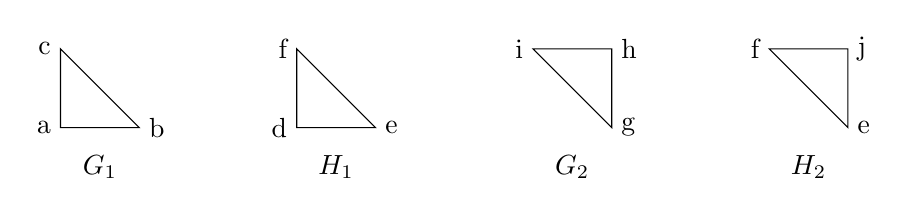
\begin{tikzpicture}
		\draw (0,0) node[left] {a} -- (1,0) node[right] {b} -- (0,1) node[left] {c} -- cycle;
		\draw (0.5,-0.5) node {$G_1$};
		\draw (3,0) node[left] {d} -- (4,0) node[right] {e} -- (3,1) node[left] {f} -- cycle;
		\draw (3.5,-0.5) node {$H_1$};
		\draw (7,0) node[right] {g} -- (7,1) node[right] {h} -- (6,1) node[left] {i} -- cycle;
		\draw (6.5,-0.5) node {$G_2$};
		\draw (10,0) node[right] {e} -- (10,1) node[right] {j} -- (9,1) node[left] {f} -- cycle;
		\draw (9.5,-0.5) node {$H_2$};
	\end{tikzpicture}
\end{center}

We can see that $G_1$ is isomorphic to $H_1$, and $G_2$ is isomorphic to $H_2$.
However, $G_1 \cup G_2$ is not isomorphic to $H_1 \cup H_2$, as shown in the figure below:
\begin{center}
	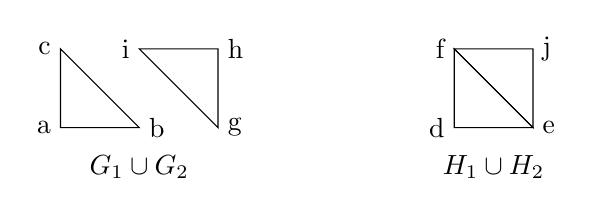
\begin{tikzpicture}
		\draw (0,0) node[left] {a} -- (1,0) node[right] {b} -- (0,1) node[left] {c} -- cycle;
		\draw (2,0) node[right] {g} -- (2,1) node[right] {h} -- (1,1) node[left] {i} -- cycle;
		\draw (1,-0.5) node {$G_1 \cup G_2$};
		\draw (5,0) node[left] {d} -- (6,0) node[right] {e} -- (5,1) node[left] {f} -- cycle;
		\draw (6,0) -- (6,1) node[right] {j} -- (5,1) -- cycle;
		\draw (5.5,-0.5) node {$H_1 \cup H_2$};
	\end{tikzpicture}
\end{center}

\end{proof}

\section*{Q.12}

\textbf{$L(G)$ is connected:}

\begin{proof}
$ $

Let $(u_1, v_1)$ and $(u_2, v_2)$ be two arbitrary vertices in $L(G)$.
Then there are two edges $u_1 \rightarrow v_1$ and $u_2 \rightarrow v_2$ in $G$.
Since $G$ is connected, we can find a path from $v_1$ to $u_2$, and we add the two edges to the path, then we have a path: $u_1 \rightarrow v_1 \rightarrow e_1 \rightarrow \cdots \rightarrow e_n \rightarrow u_2 \rightarrow v_2$.
Then we can find a corresponding path in $L(G)$: $(u_1, v_1) \rightarrow (v_1, e_1) \rightarrow \cdots \rightarrow (e_n, u_2) \rightarrow (u_2, v_2)$.
Because $(u_1, v_1)$ and $(u_2, v_2)$ are arbitrary, there is a path between any two vertices in $L(G)$.
Therefore, $L(G)$ is connected.
\end{proof}

\textbf{$L(G)$ has an Euler circuit:}

Since $G$ is regular, let the degree of each vertex be $k$.
If $k=0$, then $G$ has no edge, and $L(G)$ has no vertex, then $L(G)$ has an Euler circuit.
If $k=1$, then $G$ has two vertices and one edge, and $L(G)$ has one vertex and no edge, then $L(G)$ has an Euler circuit.
When $k \geq 2$, for each edge $e$ in $G$, both of its endpoints have degree $k$, then the number of edges sharing the same endpoint is $2k - 2$.
Then in $L(G)$, each vertex has degree $2k - 2$, which is even.
Hence, $L(G)$ has an Euler circuit.

\section*{Q.13}

Since the graph is a simple planar graph, we can use Euler's formula $v-e+r=2$.
Because there is no simple circuits of length 4 or less, we have $2e  = \sum_{\text{all region r}} deg(r) \geq 5r$.
Then $v-e+r = 2 \leq v - e + \frac{2e}{5} = v - \frac{3e}{5}$.
We can re-arrange the inequality to get $e \leq \frac{5}{3}v - \frac{10}{3}$.

\section*{Q.14}

\subsection*{(1)}

In $K_6$, each vertex is connected to other 5 vertices.
Hence, the minimum distance between any two vertices is 1.
Then the radius of $K_6$ is 1, and the diameter of $K_6$ is 1.

\subsection*{(2)}

In $K_{4,5}$, each vertex in the same partition is directly connected to all vertices in the other partition.
Hence, the minimum distance between any two vertices of the same partition is 2, since we need to go through a vertex in the other partition then go back.
The minimum distance between any two vertices of different partitions is 1.
Then the radius of $K_{4,5}$ is 2, and the diameter of $K_{4,5}$ is 2.

\subsection*{(3)}

In $Q_3$, the distance between any two vertices is the number of different bits in their binary representation.
Hence, for any two vertices, the minimum distance is 1, and the maximum distance is 3.
Then the radius of $Q_3$ is 3, and the diameter of $Q_3$ is 3.

\subsection*{(4)}

In $C_6$, the maximum distance between any two vertices is 3 when the two vertices are on the opposite sides of the cycle.
Then the radius of $C_6$ is 3, and the diameter of $C_6$ is 3.

\section*{Q.15}

We can partition the graph into two subgraphs where each subgraph contains a set of vertices of degree $1,2,3,\cdots, n$.
For each subgraph, connect all points as a list: $v_1 \leftrightarrow v_2 \leftrightarrow v_3 \leftrightarrow \cdots \leftrightarrow v_n$.
Then for the vertices with degree $k \geq 2$, connect the corresponding two vertices in the two subgraphs with $k-2$ edges.
Finally, connect the two vertices with degree $n$ in the two subgraphs with one more edge.

This is correct because:
When $n = 1$, we have two vertices with one edge connecting them, which satisfies the requirement.
When $n \geq 2$, we have:
For the first vertex, it is connected to the second vertex in the same subgraph.
Hence, it always has degree $1$.
For the last vertex, it is connected to the previous vertex in the same subgraph, and it is connected to the corresponding vertex in the other subgraph with $n - 2 + 1 = n - 1$ edges.
Hence, it always has degree $n$.
For the vertices in the middle on the $k$-th position, they are connected to the previous and the next vertex in the same subgraph, and they are connected to the corresponding vertex in the other subgraph with $k - 2$ edges.
Hence, they always have degree $k$.
And the graph is always connected, because each subgraph is connected as a list, and there is one edge connecting the two vertices of degree $n$.
Therefore, the graph satisfies the requirement.

\section*{Q.16}

\subsection*{(1)}

An n-Qube has $n \cdot 2^{n-1}$ edges.
Because each vertex has degree $n$, and there are $2^{n}$ vertices.
By the handshaking lemma, the number of edges is $n \cdot 2^{n} / 2 = n \cdot 2^{n-1}$.

\subsection*{(2)}

An n-Qube has Eular circuit if and only if $n$ is even.
This is because Eular circuit requires that each vertex has even degree, and the degree of each vertex in an $n-Qube$ is $n$.

\subsection*{(3)}

An n-Qube is always a bipartite graph.
We can partition the vertices into two sets, one set contains all vertices with even number of 1s in their binary representation, and the other set contains all vertices with odd number of 1s in their binary representation.
By the definition of $n-Qube$, only if two vertices have one different bit in their binary representation, they are connected.
Then for any two vertices, they are connected if and only if the number of 1s in their binary representation is different by 1.
Then there could only be edges between two vertices in different sets.
Within the same set, there is no edge since the difference is always even.
Hence, the $n-Qube$ is a bipartite graph.

\subsection*{(4)}

An n-Qube is a planar graph only when $n \leq 3$.

When $n = 1$, the graph is a single line, which is planar.
When $n = 2$, the graph is a square, which is planar.
When $n = 3$, the graph can be put into a plane:
\begin{center}
	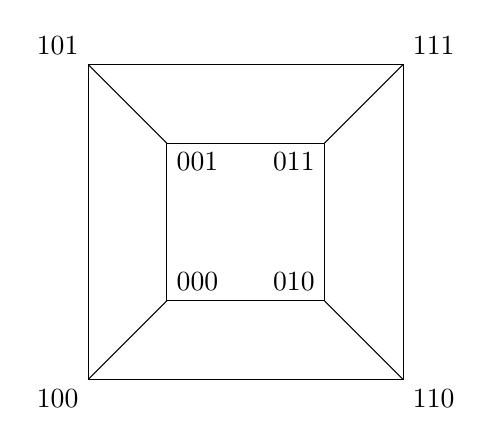
\begin{tikzpicture}
		\draw (0,0) node [above right] {000} -- (0,2) node [below right] {001} -- (2,2) node [below left] {011} -- (2,0) node [above left] {010} -- cycle;
		\draw (-1,3) node [above left] {101} -- (3,3) node [above right] {111} -- (3,-1) node [below right] {110} -- (-1,-1) node [below left] {100}  -- cycle;
		\draw (0,0) -- (-1,-1);
		\draw (0,2) -- (-1,3);
		\draw (2,2) -- (3,3);
		\draw (2,0) -- (3,-1);
	\end{tikzpicture}
\end{center}

When $n \geq 4$, the graph is not planar.
Since an n-Qube is a bipartite graph, we know the minimal length of a cycle is 4.
Then we can use the corollary of Euler's formula when the graph has no circuit of length 3 or less: $e \leq 2v - 4$.
We substitute $e$ with $n \cdot 2^{n-1}$ and $v$ with $2^{n}$, then we have:
\begin{align*}
	n \cdot 2^{n-1} &\leq 2 \cdot 2^{n} - 4 \\
	n &\leq 4 - \frac{4}{2^{n-1}} \\
\end{align*}
Since $n \geq 4$, we know that $4 \leq n \leq 4 - \frac{4}{2^{n-1}} < 4$, which is a contradiction.

\subsection*{(5)}

For $n \geq 2$, the n-Qube has a Hamilton circuit.

For $n=1$, the graph is a single line, it does have a Hamilton path but not a Hamilton circuit.
For $n \geq 2$, we can prove it by induction.

\textbf{Base case:}

When $n=2$, the graph is a square, it has a Hamilton circuit by simply selecting all edges in the square.

\textbf{Induction step:}

Suppose that for $n=k$, the n-Qube has a Hamilton circuit.
Then for $n=k+1$, we know the graph can be divided into two k-Qubes with $2^{k}$ edges connecting the two k-Qubes.
Let the first k-Qube be $G$ and the second k-Qube be $H$.

Suppose the Hamilton circuit in $G$ is $v_1 \rightarrow v_2 \rightarrow \cdots \rightarrow v_{2^{k}} \rightarrow v_1$.
Then we can take away the last edge $v_{2^{k}} \rightarrow v_1$ and the rest of the edges will form a Hamilton path in $G$.
We do this in $H$ as well, and let the Hamilton path be $u_1 \rightarrow u_2 \rightarrow \cdots \rightarrow u_{2^{k}}$.
Then we can connect $v_{2^{k}}$ and $u_{2^{k}}$ with an edge, and connect $v_1$ and $u_1$ with an edge.
Then we have a Hamilton circuit in the n-Qube: $v_1 \rightarrow v_2 \rightarrow \cdots \rightarrow v_{2^{k}} \rightarrow u_{2^{k}} \rightarrow u_{2^{k}-1} \rightarrow \cdots \rightarrow u_1 \rightarrow v_1$.
\section*{Q.17}

\subsection*{(1)}

The graph $G$ is a bipartite, since it is the planar graph for the 3-Qube, and we have proved that the 3-Qube is a bipartite graph in Q.16(3).
The graph $H$ is not a bipartite, if we look at the left 4 vertices:
\begin{center}
	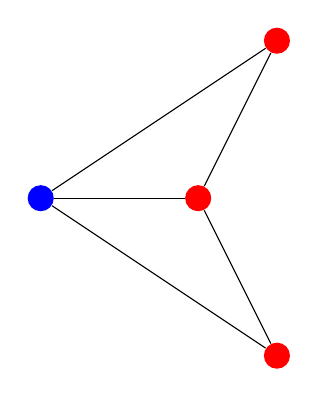
\begin{tikzpicture}
		\draw (0,0) node [circle, fill=blue] (A) {};
		\draw (2,0) node [circle, fill=red] (B) {};
		\draw (3,2) node [circle, fill=red] (C) {};
		\draw (3,-2) node [circle, fill=red] (D) {};
		\draw
		(A) edge (B)
		(A) edge (C)
		(A) edge (D)
		(B) edge (C)
		(B) edge (D);
	\end{tikzpicture}
\end{center}

If we color the leftmost vertex blue, then the other three vertices are red.
However, there are edges between the other three red vertices, which violates the definition that bipartite graph can be 2-colored.

\subsection*{(2)}

No, they are not isomorphic.
Because in graph $G$ there are no circuits of length 3, but in graph $H$ there are.

\subsection*{(3)}

No, they don't have Eular circuits.
This is because in both graphs, each vertex has degree 3, which is odd.

\section*{Q.18}

We can translate this problem into a graph problem:
There are 17 vertices, each vertex represents a student.
And there is an edge between any two vertices, represents that the two students communicate with each other.
Each edge can be colored into one of the three colors, represents that the two students can discuss one of the three problems.
To prove there are at least three students who are pairwise discussing the same problem, we can prove that there is a triangle with three edges of the same color.

\begin{proof}
$ $

Let $v$ be an arbitrary vertex in the graph.
Then there are 16 edges connected to $v$.
By the pigeonhole principle, there are at least 6 vertices that are connected to $v$ with the same color.
Without loss of generality, let the color be red.

If there is a red edge between any two vertices connected to $v$, then we have a triangle with three red edges.

If none of all edges between these 6 vertices is colored in red, then we need to color a complete graph of 6 vertices with two colors.
We can pick one vertex from the 6 vertices, and there are 5 edges connected to it.
By the pigeonhole principle, there are at least 3 edges that are colored in the same color.
Without loss of generality, let the color be blue.
If there is a blue edge between any two vertices connected to the vertex we picked, then we have a triangle with three blue edges.
If all edges between these 3 vertices are not colored in blue, then these 3 vertices are connected to each other with same color.

In all, there is a triangle with three edges of the same color.
\end{proof}

\section*{Q.19}

The number of edges in $K_{m,n}$ is $m \cdot n$.
And the number of edges in a tree with $m+n$ vertices is $m+n-1$.
Hence, $m \cdot n = m+n-1$.
Then $(m-1)(n-1) = 0$.
Since $m$ and $n$ are positive integers, we know that $m = 1$ or $n = 1$.

\section*{Q.20}

\subsection*{(a)}

The equivalent expression is $((9 / 3) + 5) * (7 - 2) = 40$.

\subsection*{(b)}

The equivalent expression is $((3 * 2) \uparrow 2) - ((5-3)*(8/4)) = 32$.

\section*{Q.21}

\subsection*{a)}

The number of different spanning trees in $K_3$ is 3.
By excluding one edge, we can get a spanning tree, and the number of edges we can exclude is 3.
Hence, the number of different spanning trees in $K_3$ is 3.

\subsection*{b)}

The spanning tree in $K_4$ has 3 edges.
We can pick 3 edges from the 6 edges in $K_4$, then exclude the situation where the 3 edges form a cycle.
Hence, the number of different spanning trees in $K_4$ is $\binom{6}{3} - 4 = 16$.

\subsection*{c)}

The spanning tree in $K_{2,2}$ can be formed by excluding one edge from the 4 edges in $K_{2,2}$.
Hence, the number of different spanning trees in $K_{2,2}$ is 4.

\subsection*{d)}

The number of different spanning trees in $C_5$ is 5.
We can exclude one edge from the 5 edges in $C_5$ to form a spanning tree.
Hence, the number of different spanning trees in $C_5$ is 5.

\section*{Q.22}

\subsection*{a)}

There is only one non-isomorphic spanning tree in $K_3$.
Since all three possible spanning trees is a tree with 3 vertices and 2 edges, then they can all be mapped to:
\begin{center}
	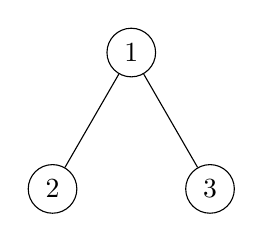
\begin{tikzpicture}
		\draw (0,0) node [circle, draw] (2) {2};
		\draw (2,0) node [circle, draw] (3) {3};
		\draw (1,1.732) node [circle, draw] (1) {1};

		\draw 
		(2) edge (1)
		(3) edge (1);
	\end{tikzpicture}
\end{center}

\subsection*{b)}

There are two non-isomorphic spanning trees in $K_4$.
The first one is:
\begin{center}
	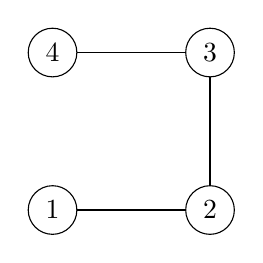
\begin{tikzpicture}
		\draw (0,0) node [circle, draw] (1) {1};
		\draw (2,0) node [circle, draw] (2) {2};
		\draw (2,2) node [circle, draw] (3) {3};
		\draw (0,2) node [circle, draw] (4) {4};

		\draw 
		(1) edge (2)
		(2) edge (3)
		(3) edge (4);
	\end{tikzpicture}
\end{center}

The second one is:
\begin{center}
	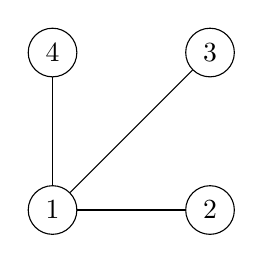
\begin{tikzpicture}
		\draw (0,0) node [circle, draw] (1) {1};
		\draw (2,0) node [circle, draw] (2) {2};
		\draw (2,2) node [circle, draw] (3) {3};
		\draw (0,2) node [circle, draw] (4) {4};

		\draw 
		(1) edge (2)
		(1) edge (4)
		(1) edge (3);
	\end{tikzpicture}
\end{center}

\subsection*{c)}

There are 3 non-isomorphic spanning trees in $K_5$.

The first one is:
\begin{center}
	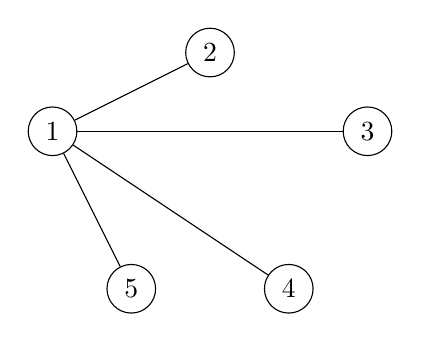
\begin{tikzpicture}
		\draw (0,0) node [circle, draw] (1) {1};
		\draw (2,1) node [circle, draw] (2) {2};
		\draw (4,0) node [circle, draw] (3) {3};
		\draw (3,-2) node [circle, draw] (4) {4};
		\draw (1,-2) node [circle, draw] (5) {5};

		\draw 
		(1) edge (2)
		    edge (3)
			edge (4)
			edge (5);
	\end{tikzpicture}
\end{center}

The second one is:
\begin{center}
	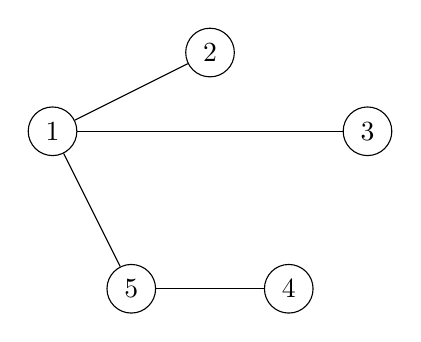
\begin{tikzpicture}
		\draw (0,0) node [circle, draw] (1) {1};
		\draw (2,1) node [circle, draw] (2) {2};
		\draw (4,0) node [circle, draw] (3) {3};
		\draw (3,-2) node [circle, draw] (4) {4};
		\draw (1,-2) node [circle, draw] (5) {5};

		\draw 
		(1) edge (2)
		    edge (3)
			edge (5)
		(4)	edge (5);
	\end{tikzpicture}
\end{center}

The second one is:
\begin{center}
	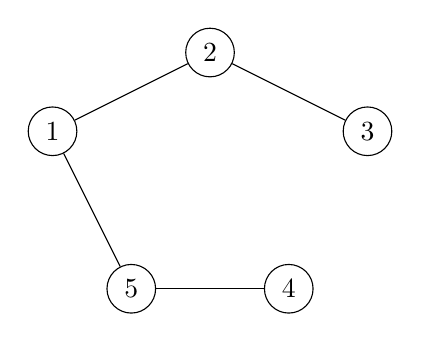
\begin{tikzpicture}
		\draw (0,0) node [circle, draw] (1) {1};
		\draw (2,1) node [circle, draw] (2) {2};
		\draw (4,0) node [circle, draw] (3) {3};
		\draw (3,-2) node [circle, draw] (4) {4};
		\draw (1,-2) node [circle, draw] (5) {5};

		\draw 
		(1) edge (2)
		(2) edge (3)
		(1)	edge (5)
		(4)	edge (5);
	\end{tikzpicture}
\end{center}

\section*{Q.23}

\subsection*{(1)}

\begin{center}
	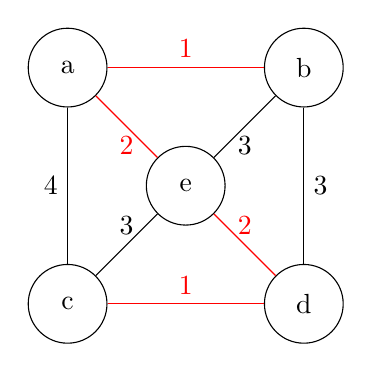
\begin{tikzpicture}
		\draw (0,0) node [circle, draw, minimum size=1cm] (a) {a};
		\draw (3,0) node [circle, draw, minimum size=1cm] (b) {b};
		\draw (0,-3) node [circle, draw, minimum size=1cm] (c) {c};
		\draw (3,-3) node [circle, draw, minimum size=1cm] (d) {d};
		\draw (1.5,-1.5) node [circle, draw, minimum size=1cm] (e) {e};

		\draw 
		(a) edge [color=red] node [above] {1} (b)
		(a) edge node [left] {4} (c)
		(a) edge [color=red] node [below] {2} (e)
		(b) edge node [right] {3} (d)
		(b) edge node [below] {3} (e)
		(c) edge node [above] {3} (e)
		(c) edge [color=red] node [above] {1} (d)
		(d) edge [color=red] node [above] {2} (e);
		;
	\end{tikzpicture}
\end{center}

\begin{center}
	\begin{tabular}{ccc}
		\toprule
		Edge & Weight & Order \\
		\midrule
		ab & 1 & 1 \\
		ae & 2 & 2 \\
		de & 2 & 3 \\
		cd & 1 & 4 \\
		\bottomrule
	\end{tabular}
\end{center}

\subsection*{(2)}

\begin{center}
	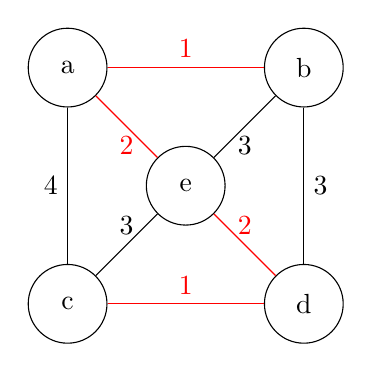
\begin{tikzpicture}
		\draw (0,0) node [circle, draw, minimum size=1cm] (a) {a};
		\draw (3,0) node [circle, draw, minimum size=1cm] (b) {b};
		\draw (0,-3) node [circle, draw, minimum size=1cm] (c) {c};
		\draw (3,-3) node [circle, draw, minimum size=1cm] (d) {d};
		\draw (1.5,-1.5) node [circle, draw, minimum size=1cm] (e) {e};

		\draw 
		(a) edge [color=red] node [above] {1} (b)
		(a) edge node [left] {4} (c)
		(a) edge [color=red] node [below] {2} (e)
		(b) edge node [right] {3} (d)
		(b) edge node [below] {3} (e)
		(c) edge node [above] {3} (e)
		(c) edge [color=red] node [above] {1} (d)
		(d) edge [color=red] node [above] {2} (e);
		;
	\end{tikzpicture}
\end{center}

\begin{center}
	\begin{tabular}{ccc}
		\toprule
		Edge & Weight & Order \\
		\midrule
		ab & 1 & 1 \\
		cd & 1 & 2 \\
		de & 2 & 3 \\
		ae & 2 & 4 \\
		\bottomrule
	\end{tabular}
\end{center}
\end{document}